\section{Evaluation}
\label{sec:evaluation}

\subsection{Protocol}
\label{sec:protocol}

The reference is Mixbox~2.0 \texttt{lerpFloat} on the sRGB display-value float path. The metric is CIEDE2000 with $k_{L}=k_{C}=k_{H}=1$, validated as described in \cref{sec:reference}. Random-set means are reported with bootstrap 95\% confidence intervals (1000 resamples, fixed resampling stream so that the reported intervals are reproducible). The perceptual scale of $\Delta E_{00}$ is used only qualitatively: below 1 is near the threshold of detection, 1--2 is visible on close inspection, 2--4 is clearly visible, and above 4 is a substantial difference.

The design targets for the repair layer are a mean $\Delta E_{00}$ below 5 and a maximum not exceeding 15 on the dark-plus-white suites. The main suites (T1--T3) are not designed to meet the maximum target, because pairs with a large lightness gap and hue opposition dominate their maxima; we report the maxima without treating them as acceptance criteria.

\subsection{Test Sets and Split}
\label{sec:sets}

\Cref{tab:sets} summarizes the test sets; \cref{app:suite} gives their exact construction, colors, $\alpha$ grids, and seeds.

\begin{table}[t]
\centering
\footnotesize
\setlength{\tabcolsep}{3pt}
\caption{Evaluation test sets.}
\label{tab:sets}
\begin{tabular}{p{0.16\linewidth}p{0.46\linewidth}rr}
\toprule
Set & Content & $n$ & Role \\
\midrule
T1 palette & all pairs of the preset palette ($10$ bases $\times$ $8$ tints) $\times$ $\alpha\in\{0.25,0.5,0.75\}$ & 240 & in-sample \\
T2 stress pairs & complementary 3, RYB mismatch 6, white/black 6, similar 4, each $\times$ 3 $\alpha$ & 57 & in-sample \\
T3 random & uniform sRGB pairs $\times$ $\alpha\in[0,1]$, fixed seed & 2000 & mixed \\
T4 identity & 10 colors $\times$ $\alpha\in\{0,1\}$ self-mixing & 20 & structural \\
T5 dark + white & 20 fixed deep colors $+$ 24 random $\times$ 9 $\alpha$ levels & 396 & in-sample \\
T5-heldout & random deep colors (fresh seed 20260812) $\times$ 9 $\alpha$ levels & 216 & held-out \\
tail & T5 fixed colors $\times$ $\alpha\in[0.92,0.99]$ $+$ blind-spot colors $\times$ full $\alpha$ & 241 & in-sample \\
T5E two-sided tail & chromatic deep colors $\times$ deep-side $\alpha$ $+$ near-neutral deep colors $\times$ both sides & 240 & in-sample \\
\bottomrule
\end{tabular}
\end{table}

The fitting corpus contains T1, T2, T5, T5E, the tail set, and the first 800 pairs of T3 (seed 20260808). Held-out data are the disjoint T3 slice $[800,2000)$, two independent T3 draws (seeds 20260809 and 20260811, disjoint from every fitting seed), and T5-heldout (fresh seed 20260812). T3 uses a deterministic PRNG (mulberry32), so all draws are reproducible.

T5E covers the two tails that the other suites leave sparse: $\alpha\in\{0.001,\dots,0.1\}$ for 20 chromatic deep colors and 12 near-neutral deep colors, and $\alpha\in\{0.92,\dots,0.99\}$ for the same near-neutral colors. The near-neutral group has a chroma range below the gate threshold and is therefore mixed by the core alone; T5E supervises the $\varphi$ map in that region.

\subsection{Results}
\label{sec:results}

\Cref{tab:insample} reports in-sample results and \cref{tab:heldout} held-out results; \cref{fig:errhist} shows the error distributions.

\begin{table}[t]
\centering
\footnotesize
\setlength{\tabcolsep}{3pt}
\caption{In-sample results against Mixbox~2.0 ($\Delta E_{00}$ mean / max). T3(fit) is the first 800 pairs of the seed-20260808 draw.}
\label{tab:insample}
\begin{tabular}{lcccccc}
\toprule
Model & T1 & T2 & T3(fit) & T5 & tail & T4 \\
\midrule
PBM & \textbf{3.286 / 15.0} & \textbf{2.667 / 10.7} & \textbf{2.759 / 15.5} & \textbf{2.258 / 7.3} & \textbf{1.678 / 8.0} & 0.00000 \\
RGB interpolation & 5.053 / 39.0 & 5.526 / 39.4 & 3.374 / 27.5 & 8.127 / 20.9 & 5.878 / 20.6 & pass \\
K--M (display-value) & 4.867 / 27.4 & 5.199 / 25.2 & 3.964 / 23.7 & 10.299 / 23.6 & 9.877 / 24.1 & pass \\
\bottomrule
\end{tabular}
\end{table}

\begin{table}[t]
\centering
\footnotesize
\setlength{\tabcolsep}{3pt}
\caption{Held-out results against Mixbox~2.0 ($\Delta E_{00}$ mean / max; bootstrap 95\% CI for the PBM mean in the note).}
\label{tab:heldout}
\begin{tabular}{lcccc}
\toprule
Model & T3 slice $[800,2000)$ & T3 seed 09 & T3 seed 11 & T5-heldout \\
\midrule
PBM & \textbf{2.789 / 19.4} & \textbf{2.719 / 23.8} & \textbf{2.852 / 22.2} & \textbf{2.377 / 9.9} \\
RGB interpolation & 3.456 / 36.8 & 3.273 / 34.5 & 3.425 / 34.6 & 7.612 / 17.1 \\
K--M (display-value) & 4.002 / 31.5 & 3.918 / 31.4 & 4.010 / 32.8 & 9.517 / 17.3 \\
\bottomrule
\end{tabular}

\smallskip
{\scriptsize Bootstrap 95\% CI (mean), PBM: slice [2.662, 2.930]; seed 09 [2.612, 2.834]; seed 11 [2.742, 2.974]; T5-heldout [2.237, 2.540].}
\end{table}

\begin{figure}[t]
\centering
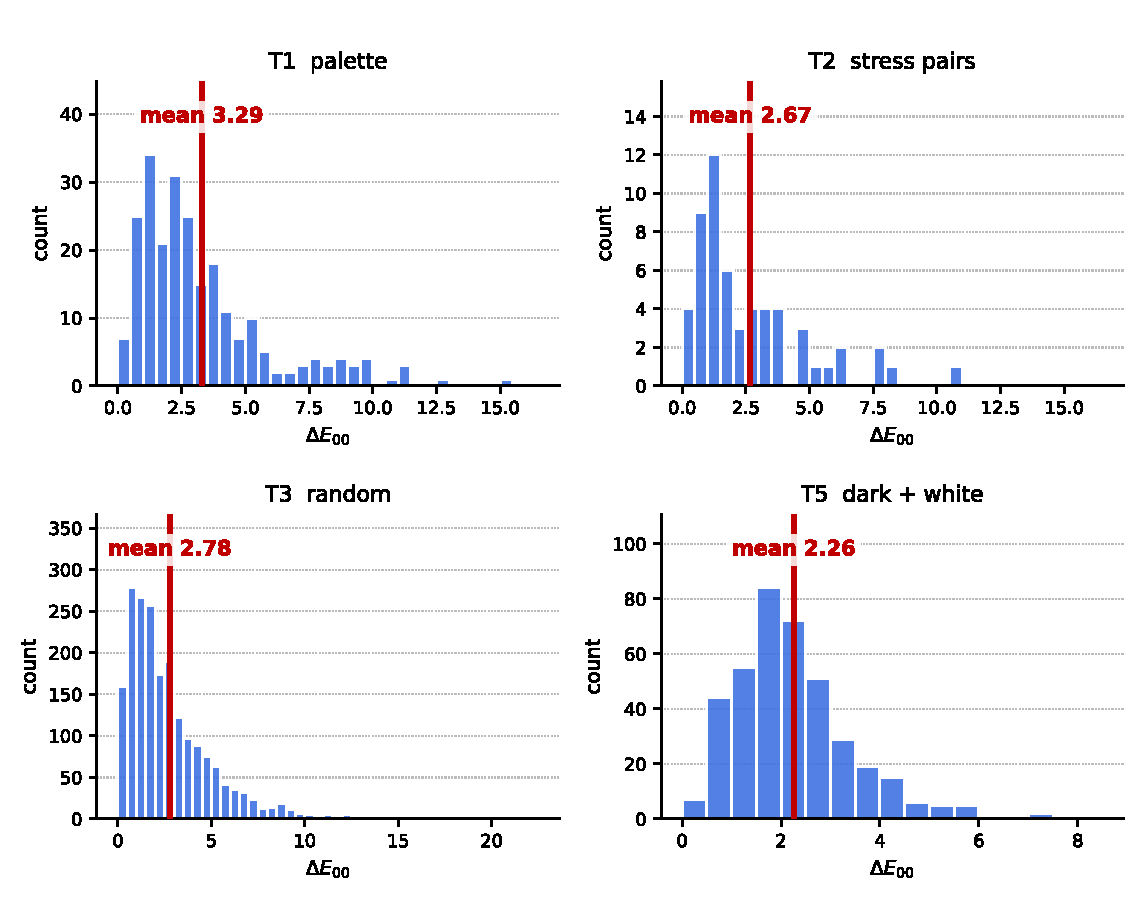
\includegraphics[width=0.72\linewidth]{fig4-error-dist.pdf}
\caption{$\Delta E_{00}$ histograms of PBM against Mixbox~2.0 on T1, T2, T3 (seed 20260808, $n=2000$), and T5 (bin width 0.5; red line: mean).}
\label{fig:errhist}
\end{figure}

Three observations follow. First, the held-out means differ from the fitting draw by at most 0.09 $\Delta E_{00}$ (T3 slice 2.789 versus 2.759), and the independent draws (2.719 and 2.852) lie in the same band. We find no evidence of overfitting under this protocol. Second, the held-out maxima (19.4--23.8) occur in random pairs that combine a large lightness gap with hue opposition; that family is the dominant source of large errors (\cref{sec:errors}). Third, the dark-plus-white repair generalizes: T5-heldout measures 2.377, 0.12 above the in-sample T5 mean, whereas RGB interpolation (7.61) and raw K--M (9.52) remain at their in-sample levels.

On T5E (240 samples), PBM measures a mean of 2.441, a maximum of 9.5, and a 95th percentile of 8.08, inside the design targets. Both applications of the $\varphi$ map improve the pairs they target: disabling the core map raises the T5E mean from 2.441 to 2.872, and disabling the map in the power-law target raises it to 2.881.

\subsection{Ablation}
\label{sec:ablation}

\Cref{tab:ablation} disables each component in the reference implementation. All variants are generated by textual patching of the algorithm source and verified to change the executed code; the tooling fails if a patch target is not found.

\begin{table}[t]
\centering
\footnotesize
\setlength{\tabcolsep}{2.5pt}
\caption{Ablation study ($\Delta E_{00}$ mean / max). T3 is the full seed-20260808 draw ($n=2000$).}
\label{tab:ablation}
\begin{tabular}{lccccc}
\toprule
Configuration & T1 & T2 & T3 & T5 & tail \\
\midrule
PBM (full) & \textbf{3.286 / 15.0} & \textbf{2.667 / 10.7} & \textbf{2.777 / 19.4} & \textbf{2.258 / 7.3} & \textbf{1.678 / 8.0} \\
$-$ cross-channel matrix $\Mthree$ & 3.674 / 23.8 & 3.534 / 14.9 & 3.218 / 25.6 & 2.259 / 7.3 & 1.678 / 8.0 \\
$-$ mutual absorption $\beta$ & 3.409 / 12.9 & 2.603 / 10.2 & 2.904 / 19.4 & 2.262 / 7.3 & 1.678 / 8.0 \\
$-$ channel coupling & 3.797 / 15.0 & 2.978 / 10.7 & 3.857 / 30.9 & 8.834 / 19.7 & 4.670 / 19.7 \\
$-$ directional responses & 3.491 / 15.0 & 2.741 / 10.7 & 2.969 / 24.2 & 4.739 / 15.2 & 3.429 / 12.4 \\
$-$ harmonic correction ($\hat{\gamma}$) & 3.649 / 15.3 & 3.543 / 13.5 & 2.890 / 20.0 & 2.258 / 7.3 & 1.678 / 8.0 \\
$-$ power-law repair ($g\equiv0$) & 3.700 / 15.0 & 3.091 / 10.7 & 3.248 / 20.4 & 9.823 / 23.8 & 8.448 / 24.0 \\
power-law everywhere ($g\equiv1$) & 4.785 / 25.2 & 5.237 / 24.4 & 2.967 / 26.1 & 2.248 / 7.3 & 1.654 / 8.0 \\
\bottomrule
\end{tabular}
\end{table}

The power-law repair and the channel coupling remain the two largest contributors on the dark-plus-white suite: T5 rises from 2.258 to 9.823 without the repair and to 8.834 without coupling. Coupling is also the strongest single term on the main suites (T3 2.777 to 3.857). The cross-channel matrix is second strongest on the main suites (T1 3.286 to 3.674; T2 2.667 to 3.534) and neutral on T5, where the repair dominates. Directional responses matter on T5 (4.739) and at the tail (3.429). Mutual absorption has a small, mixed effect: T2 improves without it (2.603) while T1 degrades (3.409), so it is retained. The harmonic correction improves all three main suites (T1 3.649 to 3.286; T2 3.543 to 2.667; T3 2.890 to 2.777) and is now a monotonically beneficial component. Forcing the power-law target everywhere degrades the main suites (T1 4.785, T2 5.237), so the gate's region selection is necessary.

\subsection{Error Structure}
\label{sec:errors}

The largest errors concentrate in pairs that combine a large lightness gap with hue opposition. The T1 worst pair is near-black $\#141417$ with orange $\#FF7A2A$ at $\alpha=0.25$ ($\Delta E_{00}=15.02$); the T2 worst pair is yellow $\#FFD61A$ with ultramarine $\#2E5EFF$ at $\alpha=0.75$ (10.70); the T3 worst pair is pale green-gray $\#C8D098$ with blue-violet $\#3A45E6$ at $\alpha\approx0.32$ (19.43). These are mixtures in which the reference's seven-dimensional latent space produces cross-channel correlations that a per-channel independent form cannot represent. Over $\alpha\in[0.05,0.95]$, the eight anchor pairs measure mean $\Delta E_{00}$ 2.85 (yellow $\times$ deep blue $\#FFC400+\#000F3D$), 3.16 (yellow $\times$ near-boundary $\#FFC400+\#000724$), 5.20 (red $\times$ green $\#A30000+\#00B359$), 7.04 (red $\times$ cyan $\#A30000+\#00D5C0$), 1.79 (magenta $\times$ green $\#E33BA8+\#00B359$), 3.80 (orange $\times$ blue $\#FF7A1A+\#2E5EFF$), 9.73 (orange $\times$ deep blue $\#FF7A1A+\#001B75$), and 5.07 (red $\times$ deep blue $\#A30000+\#001B75$), compared with a substantially larger error when the harmonic correction is removed (\cref{tab:ablation}).

On T5, the worst fixed-color pair is the dark violet $\#080248$ mixed with white at $\alpha=0.4$ ($\Delta E_{00}=7.3$); among the random deep colors the worst case is 7.3 as well. The two near-black reds in T5 ($\#280501$ and $\#250903$) measure a mean of 2.80 and a maximum of 4.14 over $\alpha\in[0.1,0.9]$ with the range gate; disabling the gate raises these values to 15.76 and 19.04. \Cref{fig:white,fig:worst} show the deep-plus-white trajectories and the worst pairs.

\begin{figure}[t]
\centering
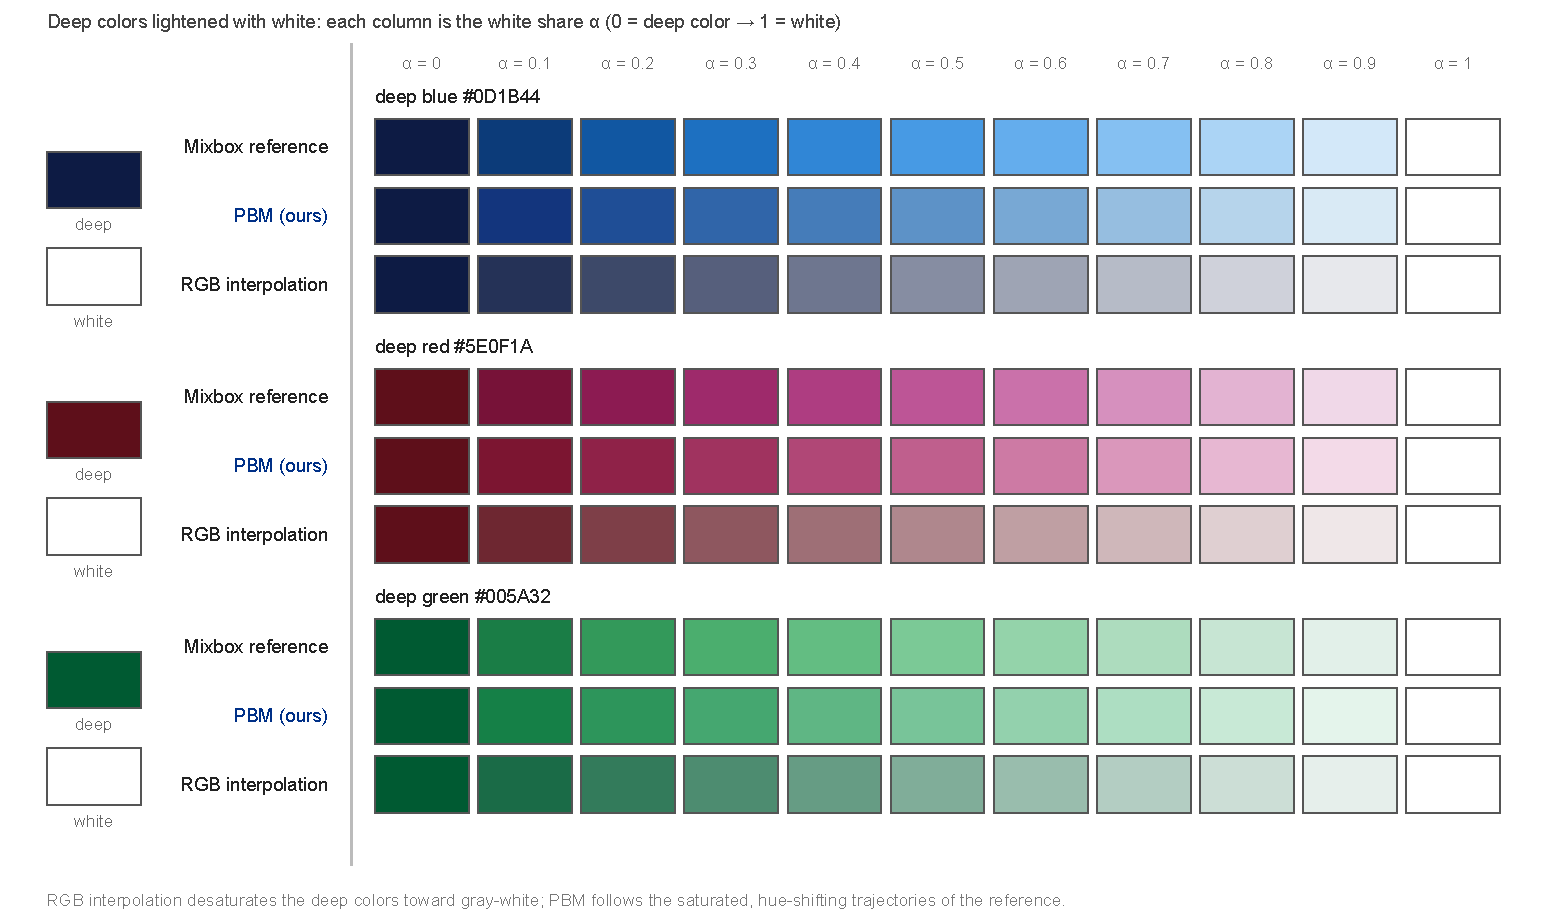
\includegraphics[width=\linewidth]{fig7-mixing-white.pdf}
\caption{Deep colors lightened with white. Each column is the white share $\alpha$ ($0$ = deep color, $1$ = white). RGB interpolation desaturates toward gray-white; PBM follows the chromatic, hue-shifting trajectories of the reference.}
\label{fig:white}
\end{figure}

\begin{figure}[t]
\centering
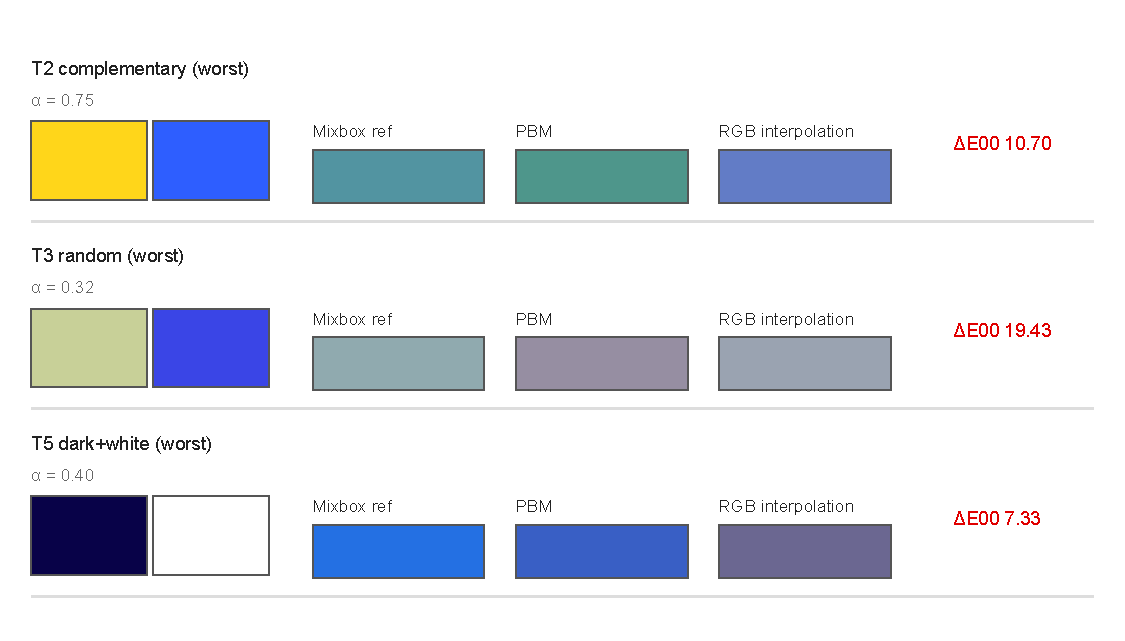
\includegraphics[width=0.82\linewidth]{fig5-worst-pairs.pdf}
\caption{Worst pairs of the T2 complementary, T3 random, and T5 dark-plus-white suites: inputs, Mixbox reference output, PBM output, RGB interpolation output, and $\Delta E_{00}$.}
\label{fig:worst}
\end{figure}

\subsection{Continuity and Exchange Symmetry}
\label{sec:continuity}

The continuity probe perturbs each channel of each input by $\pm1/255$ and the ratio by $+0.004$ for 4000 random pairs and records the largest change in the output $\Delta E_{00}$. The maximum single-step change is 1.388, with zero exceedances of 1.53. The chroma attenuation is necessary for this result: with $\mathrm{cSat}\equiv1$ the same probe measures 2.531 with 14 exceedances, because the ratio features have large gradients near the achromatic axis. \Cref{fig:continuity} shows the response for one deep-blue/white mix.

Exchange symmetry was measured on 5000 random pairs with seed 20260808. The maximum RGB difference between $F(\cb,\ct,\alpha)$ and $F(\ct,\cb,1-\alpha)$ is $6.7\times10^{-16}$, i.e.\ floating-point rounding from the different multiplication order in the two branches.

\begin{figure}[t]
\centering
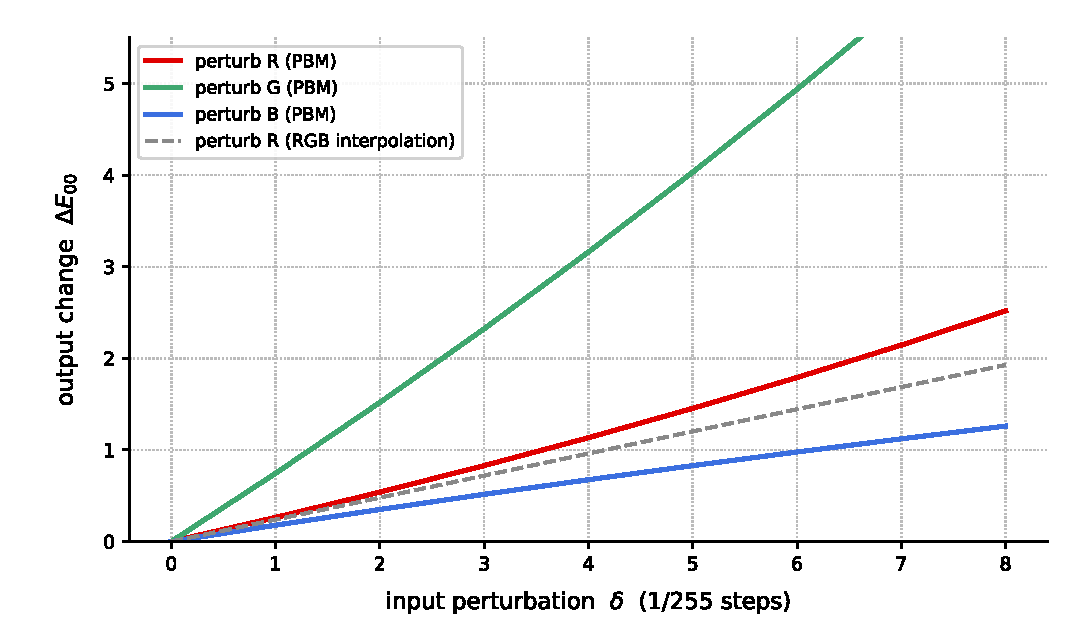
\includegraphics[width=0.72\linewidth]{fig6-continuity.pdf}
\caption{Neighborhood continuity: output change $\Delta E_{00}$ versus the input perturbation (1/255 steps on each channel of the deep blue $\#0D1B44$, mixed with white at $\alpha=0.5$); the dashed line shows the RGB interpolation response.}
\label{fig:continuity}
\end{figure}

\subsection{Runtime}
\label{sec:runtime}

\Cref{tab:runtime} reports per-mix timings measured in Node.js 26.13.1 on an AMD Ryzen~5 5600X under Windows~11. All models are loaded in the host V8 context: running the same code inside a \texttt{node:vm} sandbox inflates elementary-function calls (\texttt{Math.sqrt}, \texttt{Math.pow}) by one to two orders of magnitude---measured $8.9\times$ for PBM and $8.7\times$ for the reference---and would distort the comparison against the arithmetic-only baseline. PBM, Mixbox, and RGB interpolation use $10^{5}$ deterministic pairs and the best of nine repetitions after warm-up; the spectral K--M paths use a 50-pair subset because the iterative inversion dominates their runtime. Absolute timings are machine- and implementation-dependent; the ratios within this table are measured in one environment and are reported to support the interface argument, not as a general performance claim.

\begin{table}[t]
\centering
\small
\caption{Runtime cost per mix (best of nine repetitions after warm-up). The last column is the model's time relative to PBM.}
\label{tab:runtime}
\begin{tabular}{llrrr}
\toprule
Model & Path & ns/op & ops/s & Relative time \\
\midrule
PBM & analytic float arithmetic & 226 & 4{,}431,819 & 1.00 \\
Mixbox 2.0 & $256^{3}$ LUT lookup & 166 & 6{,}021,376 & 0.73 \\
RGB interpolation & linear blend & 16 & 63{,}572{,}791 & 0.070 \\
K--M spectral, direct & per-wavelength K/S $+$ D65$\times$CMF & 1{,}195 & 836,820 & 5.3 \\
K--M spectral, RGB-in & iterative unmix $+$ spectral mix & 22{,}400{,}000 & 45 & $9.9\times10^{4}$ \\
\bottomrule
\end{tabular}
\end{table}

PBM costs about 0.23 $\mu$s per mix, 1.4 times the reference's table lookup and 14 times a linear blend. The spectral K--M forward pipeline is not slow in itself: with pigment spectra known, the per-wavelength integration costs about 1.2 $\mu$s, roughly 5 times PBM. The obstacle is the interface: mixing two arbitrary RGB colors requires inverting each color into pigment concentrations, an iterative optimization costing about 22 ms per mix, or roughly $10^{5}$ times PBM. PBM's advantage is therefore not raw speed but the absence of a spectral representation, an inversion, or a multi-megabyte table. In interactive painting, mixing is applied per stroke or per operation rather than per rendered pixel; for per-pixel rendering, both models would be vectorized or implemented on the GPU, for which the analytic form is more portable. The absence of trigonometric and logarithmic evaluation in the harmonic correction also makes the model cheap to vectorize.

\subsection{Validation Against an Independent Synthetic Spectral World}
\label{sec:synthetic}

The evaluation above measures PBM against the reference. This section cross-validates against a ground truth computed from synthetic pigment spectra that were not used to fit PBM.

\paragraph{Dataset.}
The dataset contains 29 pigments: 24 functional hues covering the hue circle and the neutral scale, and 5 darkened derivations for the dark-plus-white suites. Each pigment is represented by separate absorption and scattering coefficients on a 10 nm grid over 380--750 nm (38 samples):
\begin{equation}
K(\lambda)=\kappa_{\mathrm{base}}+\sum_{i}A_{i}e^{-((\lambda-\mu_{i})/\sigma_{i})^{2}}
+\sum_{j}\frac{B_{j}}{1+e^{\pm((\lambda-\lambda_{j})/w_{j})}},
\qquad S(\lambda)=S_{\mathrm{base}}.
\label{eq:synthetic}
\end{equation}
Band positions are fixed by first-principles pigment chemistry (steep blue--green absorption edges for yellow/orange/red families, red-side rising edges for blue/green, a green-region band for magenta, and characteristic transition-metal or organic bands), whereas amplitudes, widths, bases, and scattering are calibrated to the publicly available BabelColor X-Rite ColorChecker Classic Avg30 spectra \cite{pascale2012} by coordinate descent (fit $\Delta E_{00}\le1.2$, most patches $\le0.2$). The ColorChecker patches are formulated color-card spectra, not pure-pigment masstone spectra; the K--M equations are closed for any reflectance spectrum, and the chart is designed for RGB displays, so no display calibration is required. The synthetic world is an approximation, not measured paint.

\paragraph{Pipeline and suites.}
The forward pipeline applies separate Duncan superposition of $K$ and $S$, evaluates \cref{eq:km} per wavelength, integrates against D65 and the CIE 1931 $2^{\circ}$ observer on the 10 nm grid, and converts to sRGB (clamping and flagging out-of-gamut samples). The inputs to all compared models are the rendered sRGB colors of the pure pigments, which avoids the issue of colors that cannot be mixed from pigments. Six suites mirror the T-suite structure: P1 (all 828 pairs of the 24-hue palette), P2 (9 stress pairs), P3 (2000 random pigment pairs, fresh seed 20260813), P5 (15 deep pigments $\times$ white), P5-buff (the same deep set $\times$ buff), and P5E (the two-sided tail grid). Out-of-gamut samples are clamped and counted.

\Cref{tab:synthetic} reports the results and \cref{fig:physical} visualizes three representative pairs.

\begin{table}[t]
\centering
\footnotesize
\setlength{\tabcolsep}{3pt}
\caption{$\Delta E_{00}$ against the synthetic-spectra reference (mean / max; bootstrap 95\% CI for random-set means in the note; out-of-gamut samples clamped and counted).}
\label{tab:synthetic}
\begin{tabular}{lcccccc}
\toprule
Model & P1 & P2 & P3 & P5 & P5-buff & P5E \\
 & {\scriptsize$n{=}828$, oog 6} & {\scriptsize$n{=}27$} & {\scriptsize$n{=}2000$, oog 35} & {\scriptsize$n{=}135$} & {\scriptsize$n{=}135$, oog 2} & {\scriptsize$n{=}150$, oog 6} \\
\midrule
PBM & 6.70 / 36.3 & 13.38 / 29.7 & 5.60 / 35.9 & 8.44 / 22.3 & 4.99 / 17.1 & 3.40 / 13.9 \\
Mixbox 2.0 & 6.46 / 31.5 & 12.71 / 24.9 & 5.10 / 30.2 & 8.86 / 25.0 & 4.56 / 18.9 & 3.39 / 20.9 \\
RGB interpolation & 6.14 / 29.5 & 11.25 / 20.4 & 4.89 / 25.4 & 8.24 / 27.0 & 5.95 / 15.8 & 3.88 / 26.9 \\
K--M display-value & 5.55 / 30.5 & 8.82 / 16.6 & 4.38 / 30.5 & 12.13 / 30.8 & 4.95 / 18.1 & 4.25 / 28.2 \\
\bottomrule
\end{tabular}

\smallskip
{\scriptsize Bootstrap 95\% CI (mean): PBM P1 [6.320, 7.045], P3 [5.390, 5.822], P5 [7.610, 9.258]; Mixbox P1 [6.080, 6.808], P3 [4.884, 5.333], P5 [7.964, 9.786].}
\end{table}

\begin{figure}[t]
\centering
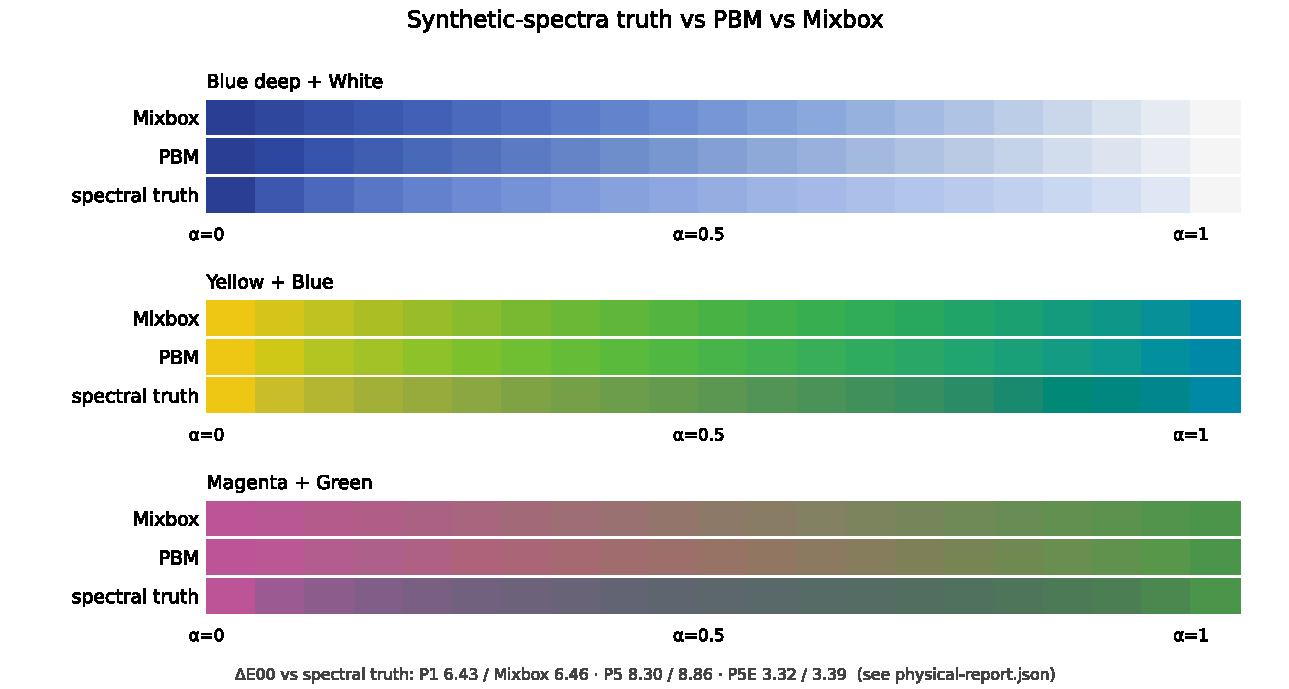
\includegraphics[width=0.88\linewidth]{fig8-physical.pdf}
\caption{Synthetic-spectra truth versus PBM and Mixbox for three representative pigment pairs (deep blue $\times$ white, yellow $\times$ blue, magenta $\times$ green) over $\alpha=0$--$1$ (21 steps).}
\label{fig:physical}
\end{figure}

Three observations follow. First, PBM and the reference are comparable on this world: the per-suite mean differences $\mathrm{PBM}-\mathrm{Mixbox}$ range from $-0.42$ (P5) to $+0.67$ (P2), and every pair of bootstrap intervals overlaps. Neither model was trained on this world, so the parity is evidence that PBM's accuracy is not an artifact of fitting the reference's outputs. PBM is closer on P5 and P5E; the reference is closer on P1, P2, P3, and P5-buff; we did not test the differences for significance. Second, the hue trajectories agree: \cref{tab:hue} reports mean and median absolute hue differences for chromatic samples ($C^{\ast}>10$). PBM's mean hue error is lower on three of the six suites (P5, P5-buff, P5E) and within $2^{\circ}$ on the others. Third, the residual per-suite mean errors (3.40--13.38 $\Delta E_{00}$) are structural: the synthetic world mixes by spectral K--M, whereas Mixbox mixes in a trained latent polynomial.

\begin{table}[t]
\centering
\small
\caption{Hue agreement with the synthetic spectral truth: mean and median absolute hue difference in degrees over chromatic samples ($C^{\ast}>10$).}
\label{tab:hue}
\begin{tabular}{lcc}
\toprule
Suite & PBM & Mixbox 2.0 \\
\midrule
P1 & 11.33 / 6.62 & 11.01 / 5.96 \\
P2 & 23.17 / 17.23 & 21.46 / 18.01 \\
P3 & 9.27 / 4.62 & 8.64 / 3.73 \\
P5 & 9.54 / 5.77 & 9.67 / 7.15 \\
P5-buff & 8.59 / 5.79 & 8.62 / 5.30 \\
P5E & 2.56 / 0.62 & 2.73 / 0.74 \\
\bottomrule
\end{tabular}
\end{table}

\paragraph{What this establishes and what it does not.}
The experiment supports two claims: (i) PBM's accuracy is not an artifact of overfitting the reference's outputs, because it matches the reference against an independent synthetic spectral world; and (ii) the qualitative behavior families---yellow $\times$ blue gives green, complementary pairs give muted colors, deep $+$ white preserves hue---also hold under two-constant spectral K--M mixing. It does not establish that PBM predicts real-paint masstone mixing, nor that it is closer to real paint than the reference. The synthetic world is itself an approximation, and PBM's relation to real paint is bounded by the reference's relation to real paint plus PBM's measured deviation from the reference.

\subsection{Threats to Validity}
\label{sec:threats}

\paragraph{Reference dependence.}
PBM is fitted to Mixbox~2.0. If the reference changes, the constants must be re-estimated with the procedure of \cref{sec:estimation}. The measured accuracy is relative to that reference; it does not bound the error against measured paint samples.

\paragraph{Synthetic world.}
The cross-validation uses two-constant K--M mixing of synthetic spectra calibrated to ColorChecker patches. Both the two-constant approximation and the patch-based calibration limit the interpretation; the synthetic world is not a substitute for measured pigment spectra.

\paragraph{Metric.}
We use CIEDE2000 with uniform weights. Other color-difference formulas or observer/illuminant choices may reorder individual pairs and change the reported means.

\paragraph{Sampling.}
Fixed suites are in-sample; only the random sets have confidence intervals. The CIs cover sampling variability of the mean, not model-selection or implementation uncertainty.

\paragraph{Scope.}
The model is defined for opaque, uniformly mixed colors in sRGB display space. It does not model layering, glazing, opacity, texture, or spectral output.
